% Work-MAT | 2. rocnik | hodina 15 | navaznost na hodiny 14 a 16
\documentclass[11pt,a4paper]{article}
\input{../../sablony/pripravy/priprava.sty}
\usepackage{tikz}
\usetikzlibrary{arrows.meta}
\nastavPripravu{2. ročník}{Exponenciální funkce}{15}{Exponenciální funkce V: průsečíky a grafické úlohy}

\begin{document}

\blok{Od sestavení předpisu k porovnávání grafů}
V minulé hodině jsme sestavovali exponenciální předpis ze zadaných bodů a vlastností grafu. Nyní budeme řešit opačnou otázku: \emph{co můžeme ze známého předpisu a grafu vyčíst?} Zajímat nás bude zejména, kdy dvě funkce nabývají stejné hodnoty a zda se jejich grafy vůbec protínají. Přitom využijeme monotónnost, asymptoty a posuny exponenciálních grafů, které již známe.

\poznamka{Nejprve společně připomenout $D(f)=\mathbb{R}$, $H(f)=(0;+\infty)$, bod $[0;1]$ a vodorovnou asymptotu základní funkce $y=a^x$. Navázat krátkou otázkou: Kdy mají dvě funkce stejnou funkční hodnotu? Odpověď ukažte na grafu, ne na algebraické úpravě.}

\begin{zadaniBox}[title={Věta - Průsečíky grafů funkcí}]
Grafy funkcí $f$ a $g$ se protínají v bodě $[x_0;y_0]$ právě tehdy, když
\[
  f(x_0)=g(x_0)=y_0.
\]
Hledat společnou hodnotu funkcí tedy znamená hledat průsečíky jejich grafů. Jejich \textbf{souřadnice $x$} jsou řešeními rovnosti $f(x)=g(x)$.
\end{zadaniBox}

\blok{Průsečík s vodorovnou přímkou}
Nejjednodušší je porovnat exponenciální funkci s konstantní funkcí $g(x)=c$. Vodorovná přímka $y=c$ ukazuje, zda a při kterém argumentu exponenciála nabývá hodnoty $c$.

\begin{prikladReseniBox}[title={Příklad 1}]
Do jedné soustavy souřadnic sestroj $f(x)=2^x$ a přímku $y=4$.
\begin{enumerate}[label=\alph*)]
  \item Vyznač jejich průsečík a urči jeho souřadnice.
  \item Urči, kdy platí $2^x<4$ a kdy $2^x>4$.
  \item Vysvětli, proč nemohou mít grafy dva různé průsečíky.
\end{enumerate}
\tcblower
Pro základní exponenciálu stačí například body $[-2;\frac{1}{4}]$, $[-1;\frac{1}{2}]$, $[0;1]$, $[1;2]$, $[2;4]$ a $[3;8]$.
\begin{enumerate}[label=\alph*)]
  \item Společný bod je $[2;4]$, protože $f(2)=2^2=4$.
  \item Pro $x<2$ je $2^x<4$; pro $x>2$ je $2^x>4$.
  \item Funkce $2^x$ přísně roste, proto hodnoty $4$ nabývá nejvýše jednou.
\end{enumerate}
\begin{center}
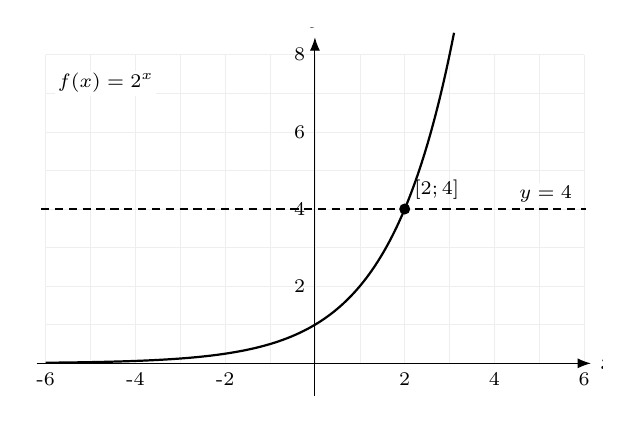
\begin{tikzpicture}[x=.57cm,y=.49cm,>=Latex]
\clip (-6.4,-1.1) rectangle (6.4,8.7);
\draw[step=1,gray!13,very thin] (-6,0) grid (6,8);
\draw[->] (-6.2,0)--(6.15,0) node[right] {$x$};
\draw[->] (0,-.85)--(0,8.45) node[above] {$y$};
\foreach \x in {-6,-4,-2,2,4,6}{\node[below,font=\scriptsize] at (\x,0) {\x};}
\foreach \y in {2,4,6,8}{\node[left,font=\scriptsize] at (0,\y) {\y};}
\draw[thick,domain=-6:3.1,samples=110,smooth] plot (\x,{pow(2,\x)});
\draw[thick,densely dashed] (-6.1,4)--(6.05,4);
\fill (2,4) circle (2pt) node[above right,font=\scriptsize] {$[2;4]$};
\node[font=\scriptsize,anchor=north west,fill=white,inner sep=1pt] at (-5.8,7.6) {$f(x)=2^x$};
\node[font=\scriptsize,anchor=south east,fill=white,inner sep=1pt] at (5.8,4.1) {$y=4$};
\end{tikzpicture}
\end{center}
\end{prikladReseniBox}

\poznamka{Žáci si graf skutečně narýsují. Doporučené osy: $x$ od $-6$ do $6$, $y$ od $0$ do $8$. Vyznačit průsečík a vodorovnou asymptotu $y=0$. Poté změnit přímku na $y=0$ a zeptat se, zda nový průsečík vznikne.}

\blok{Porovnávání dvou exponenciálních grafů}
Při porovnání dvou exponenciálních funkcí hledáme místo, kde se grafy setkají, a sledujeme, který z nich je před průsečíkem výše a který níže.

\begin{prikladReseniBox}[title={Příklad 2}]
Do jedné soustavy sestroj funkce $f(x)=2^x$ a $g(x)=\left(\frac{1}{2}\right)^x$.
\begin{enumerate}[label=\alph*)]
  \item Urči společný bod grafů.
  \item Rozhodni, která funkce nabývá větších hodnot pro $x<0$ a pro $x>0$.
  \item Porovnej jejich monotónnost a asymptoty.
\end{enumerate}
\tcblower
\begin{enumerate}[label=\alph*)]
  \item Obě funkce mají pro $x=0$ hodnotu $1$, tedy průsečík $[0;1]$.
  \item Pro $x<0$ leží výše graf $g$; pro $x>0$ leží výše graf $f$.
  \item $f$ roste, $g$ klesá; obě mají asymptotu $y=0$.
\end{enumerate}
\begin{center}
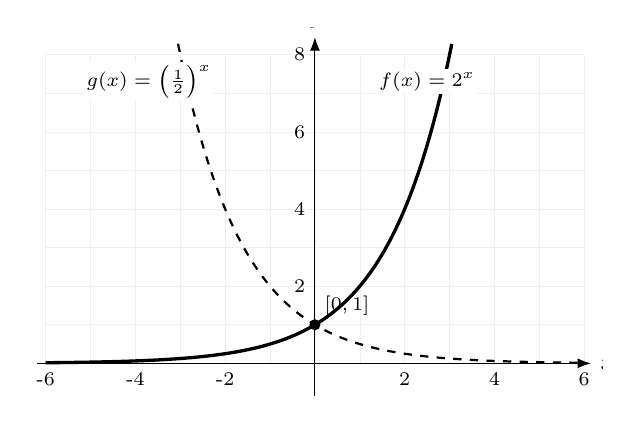
\begin{tikzpicture}[x=.57cm,y=.49cm,>=Latex]
\clip (-6.4,-1.1) rectangle (6.4,8.7);
\draw[step=1,gray!13,very thin] (-6,0) grid (6,8);
\draw[->] (-6.2,0)--(6.15,0) node[right] {$x$};
\draw[->] (0,-.85)--(0,8.45) node[above] {$y$};
\foreach \x in {-6,-4,-2,2,4,6}{\node[below,font=\scriptsize] at (\x,0) {\x};}
\foreach \y in {2,4,6,8}{\node[left,font=\scriptsize] at (0,\y) {\y};}
\draw[very thick,domain=-6:3.05,samples=110,smooth] plot (\x,{pow(2,\x)});
\draw[thick,dashed,domain=-3.05:6,samples=110,smooth] plot (\x,{pow(0.5,\x)});
\fill (0,1) circle (2pt) node[above right,font=\scriptsize] {$[0;1]$};
\node[font=\scriptsize,fill=white,inner sep=1pt] at (2.5,7.3) {$f(x)=2^x$};
\node[font=\scriptsize,fill=white,inner sep=1pt] at (-3.7,7.3) {$g(x)=\left(\frac{1}{2}\right)^x$};
\end{tikzpicture}
\end{center}
\end{prikladReseniBox}

\blok{Co se stane po posunutí grafu?}
Z třinácté a čtrnácté hodiny víme, že posun o číslo $q$ změní asymptotu z $y=0$ na $y=q$. Zároveň se změní hodnoty, kterých funkce nabývá, a tím i její případné průsečíky s vodorovnou přímkou.

\begin{prikladReseniBox}[title={Příklad 3}]
Sestroj $h(x)=2^{x-1}+1$ a vodorovné přímky $y=3$ a $y=1$.
\begin{enumerate}[label=\alph*)]
  \item Urči posun, asymptotu a obor hodnot funkce $h$.
  \item Najdi průsečík grafu s přímkou $y=3$.
  \item Rozhodni, zda se graf protne s přímkou $y=1$.
\end{enumerate}
\tcblower
\begin{enumerate}[label=\alph*)]
  \item Posun doprava o $1$ a nahoru o $1$; asymptota $y=1$, $H(h)=(1;+\infty)$.
  \item $h(2)=2^{2-1}+1=3$, tedy průsečík $[2;3]$.
  \item Žádný průsečík neexistuje, protože $h(x)>1$ pro všechna $x\in\mathbb{R}$.
\end{enumerate}
\begin{center}
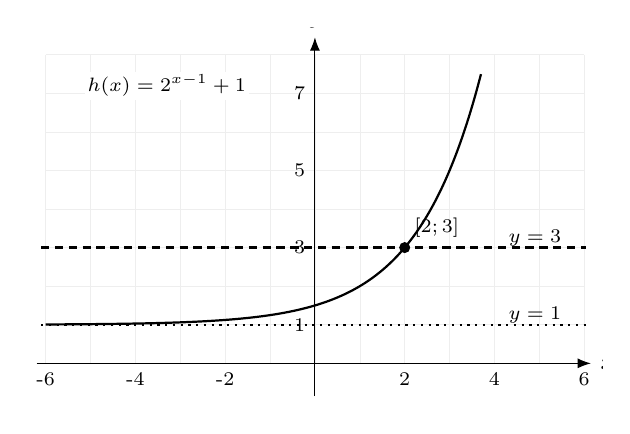
\begin{tikzpicture}[x=.57cm,y=.49cm,>=Latex]
\clip (-6.4,-1.1) rectangle (6.4,8.7);
\draw[step=1,gray!13,very thin] (-6,0) grid (6,8);
\draw[->] (-6.2,0)--(6.15,0) node[right] {$x$};
\draw[->] (0,-.85)--(0,8.45) node[above] {$y$};
\foreach \x in {-6,-4,-2,2,4,6}{\node[below,font=\scriptsize] at (\x,0) {\x};}
\foreach \y in {1,3,5,7}{\node[left,font=\scriptsize] at (0,\y) {\y};}
\draw[thick,domain=-6:3.7,samples=110,smooth] plot (\x,{pow(2,\x-1)+1});
\draw[thick,densely dashed] (-6.1,3)--(6.05,3);
\draw[thick,dotted] (-6.1,1)--(6.05,1);
\fill (2,3) circle (2pt) node[above right,font=\scriptsize] {$[2;3]$};
\node[font=\scriptsize,fill=white,inner sep=1pt] at (-3.3,7.2) {$h(x)=2^{x-1}+1$};
\node[font=\scriptsize,anchor=west] at (4.1,3.25) {$y=3$};
\node[font=\scriptsize,anchor=west] at (4.1,1.25) {$y=1$};
\end{tikzpicture}
\end{center}
\end{prikladReseniBox}

\poznamka{Žáci opět narýsují graf; doporučené osy $x\in[-6;6]$, $y\in[0;8]$. Zdůraznit, že asymptota není průsečík: graf se k přímce $y=1$ pouze přibližuje.}

\blok{Kdy přesné řešení z grafu nepřečteme?}
Někdy průsečík leží mezi body s jednoduchými souřadnicemi. Graf nám přesto umožňuje odhadnout řešení nebo prokázat, že se nachází v určitém intervalu, aniž bychom zatím znali další početní metody.

\begin{prikladReseniBox}[title={Příklad 4}]
Porovnej $f(x)=3^x$ s přímkou $y=5$.
\begin{enumerate}[label=\alph*)]
  \item Mezi kterými dvěma celými čísly leží argument jejich průsečíku?
  \item Proč je průsečík právě jeden?
  \item Má graf $y=3^x$ průsečík s přímkou $y=0$?
\end{enumerate}
\tcblower
\begin{enumerate}[label=\alph*)]
  \item $3^1=3<5<9=3^2$, a proto je hledané $x$ mezi $1$ a $2$.
  \item Funkce $3^x$ je spojitá a přísně rostoucí; hodnoty $5$ nabývá právě jednou.
  \item Ne, neboť $3^x>0$ pro každé $x\in\mathbb{R}$.
\end{enumerate}
\end{prikladReseniBox}

\begin{prikladReseniBox}[title={Příklad 5}]
Uvažuj funkce $f(x)=2^x+1$ a $g(x)=2^x+3$.
\begin{enumerate}[label=\alph*)]
  \item Rozhodni bez kreslení, zda mají grafy průsečík.
  \item Zdůvodni výsledek a načrtni oba grafy do jedné soustavy.
  \item Urči asymptoty obou funkcí.
\end{enumerate}
\tcblower
\begin{enumerate}[label=\alph*)]
  \item Průsečík nemají.
  \item Pro každé $x$ platí $g(x)=f(x)+2$; druhý graf leží stále o $2$ výše než první.
  \item Asymptoty jsou $y=1$ pro $f$ a $y=3$ pro $g$.
\end{enumerate}
\end{prikladReseniBox}

\blok{Procvičení}
\begin{zadaniReseniBox}[title={Samostatná práce 1}]
\begin{enumerate}[label=\alph*)]
  \item Sestroj $y=3^x$ a $y=9$; urči průsečík.
  \item Sestroj $y=\left(\frac{1}{2}\right)^x$ a $y=4$; urči průsečík.
  \item U funkcí $y=2^{x+1}$ a $y=8$ urči společný bod.
  \item Načrtni $y=2^x-2$ a urči průsečík s osou $x$.
  \item Zjisti, zda se $y=3^x+1$ protne s přímkou $y=1$.
  \item Porovnej $y=2^x$ a $y=\left(\frac{1}{2}\right)^x$ pro $x>0$.
  \item Rozhodni, zda se protnou grafy $y=3^x$ a $y=3^{x-1}$.
  \item Rozhodni, zda se protnou grafy $y=2^x$ a $y=2^x+1$.
  \item Urči dvě po sobě jdoucí celá čísla, mezi nimiž platí $2^x=5$.
  \item Sestroj $y=\left(\frac{1}{2}\right)^{x-1}+2$; urči asymptotu a průsečík s $y=3$.
\end{enumerate}
\tcblower
\begin{enumerate}[label=\alph*)]
  \item $[2;9]$.
  \item $[-2;4]$.
  \item $[2;8]$.
  \item $[1;0]$.
  \item Ne; obor hodnot je $(1;+\infty)$.
  \item $2^x>\left(\frac{1}{2}\right)^x$.
  \item Ne, $3^x=3\cdot3^{x-1}$; první graf leží výše.
  \item Ne, druhý graf je vždy o $1$ výše.
  \item $2<x<3$.
  \item Asymptota $y=2$; průsečík $[1;3]$.
\end{enumerate}
\end{zadaniReseniBox}

\poznamka{Samostatná práce obsahuje více úloh, než se běžně stihne v jedné hodině. Vyberte podle tempa třídy například a), b), d), e), g) a j). U náčrtků vyžadovat osu $x$, osu $y$, označenou asymptotu a alespoň tři vypočtené body.}

\begin{zadaniReseniBox}[title={Rozšíření 1}]
Rozhodni, kolikrát se může graf $f(x)=2^x$ protnout s vodorovnou přímkou $y=c$, jestliže
\begin{enumerate}[label=\alph*)]
  \item $c>0$;
  \item $c=0$;
  \item $c<0$.
\end{enumerate}
Odpověď vysvětli pomocí oboru hodnot a monotónnosti.
\tcblower
\begin{enumerate}[label=\alph*)]
  \item Právě jednou: $H(f)=(0;+\infty)$ a $f$ je prostá.
  \item Nikdy: nula do oboru hodnot nepatří.
  \item Nikdy: funkce nemá záporné hodnoty.
\end{enumerate}
\end{zadaniReseniBox}

\begin{zadaniReseniBox}[title={Rozšíření 2}]
Najdi grafickým odhadem všechna řešení rovnosti $2^x=x+2$.
\begin{enumerate}[label=\alph*)]
  \item Nakresli do jedné soustavy grafy $y=2^x$ a $y=x+2$.
  \item Jedno řešení urči přesně, druhé ohranič dvěma po sobě jdoucími celými čísly.
\end{enumerate}
\tcblower
Z grafu lze odečíst průsečík $[2;4]$, tedy řešení $x=2$. Druhý průsečík leží mezi $-2$ a $-1$, protože při $x=-2$ je $2^x=\frac{1}{4}>0=x+2$, zatímco při $x=-1$ je $2^x=\frac{1}{2}<1=x+2$.
\end{zadaniReseniBox}

\begin{zadaniReseniBox}[title={Domácí úkol}]
\begin{enumerate}[label=\alph*)]
  \item Sestroj $y=2^x$ a $y=8$; urči společný bod.
  \item Urči průsečík grafu $y=\left(\frac{1}{3}\right)^x$ s přímkou $y=9$.
  \item Urči společný bod grafů $y=2^{x-1}+2$ a $y=4$.
  \item Urči, kde se graf $y=3^x-1$ protne s osou $x$.
  \item Sestroj $y=2^x+1$ a $y=3$; vyznač průsečík a asymptotu exponenciály.
  \item Do jedné soustavy sestroj $y=2^x$ a $y=\left(\frac{1}{2}\right)^x$; vyznač průsečík a popiš vzájemnou polohu grafů.
  \item Sestroj $y=2^{x-2}+1$ a $y=2$; vyznač průsečík a asymptotu exponenciály.
  \item Vysvětli, proč nemá $2^x=-1$ reálné řešení.
  \item Rozhodni, zda se grafy $y=2^x$ a $y=2^{x+1}$ protínají, a zdůvodni.
  \item Mezi kterými dvěma po sobě jdoucími celými čísly leží řešení rovnosti $3^x=7$? Vysvětli pomocí grafu nebo funkčních hodnot.
\end{enumerate}
\tcblower
\begin{enumerate}[label=\alph*)]
  \item $[3;8]$.
  \item $[-2;9]$.
  \item $[2;4]$.
  \item $[0;0]$.
  \item $[1;3]$, asymptota $y=1$.
  \item $[0;1]$; pro $x<0$ je výše graf $\left(\frac{1}{2}\right)^x$, pro $x>0$ graf $2^x$.
  \item $[2;2]$, asymptota $y=1$.
  \item $2^x>0$ pro všechna reálná $x$.
  \item Ne; $2^{x+1}=2\cdot2^x>2^x$ pro každé $x$.
  \item $1<x<2$, protože $3<7<9$.
\end{enumerate}
\end{zadaniReseniBox}

\poznamka{Domácí úkol je sestaven na přibližně 20--30 minut. U úloh e), f) a g) trvat na skutečně narýsovaném grafu s vhodným měřítkem os a označenou asymptotou.\par\medskip\textbf{Návaznost:} V hodině 16 již přejdeme od odečítání průsečíků z grafu k početnímu řešení exponenciálních rovnic se stejným základem.}

\end{document}
